\documentclass[12pt,]{article}
\usepackage{lmodern}
\usepackage{amssymb,amsmath}
\usepackage{ifxetex,ifluatex}
\usepackage{fixltx2e} % provides \textsubscript
\ifnum 0\ifxetex 1\fi\ifluatex 1\fi=0 % if pdftex
  \usepackage[T1]{fontenc}
  \usepackage[utf8]{inputenc}
\else % if luatex or xelatex
  \ifxetex
    \usepackage{mathspec}
  \else
    \usepackage{fontspec}
  \fi
  \defaultfontfeatures{Ligatures=TeX,Scale=MatchLowercase}
\fi
% use upquote if available, for straight quotes in verbatim environments
\IfFileExists{upquote.sty}{\usepackage{upquote}}{}
% use microtype if available
\IfFileExists{microtype.sty}{%
\usepackage{microtype}
\UseMicrotypeSet[protrusion]{basicmath} % disable protrusion for tt fonts
}{}
\usepackage[margin = 1.2in]{geometry}
\usepackage{hyperref}
\PassOptionsToPackage{usenames,dvipsnames}{color} % color is loaded by hyperref
\hypersetup{unicode=true,
            colorlinks=true,
            linkcolor=black,
            citecolor=blue,
            urlcolor=black,
            breaklinks=true}
\urlstyle{same}  % don't use monospace font for urls
\usepackage{color}
\usepackage{fancyvrb}
\newcommand{\VerbBar}{|}
\newcommand{\VERB}{\Verb[commandchars=\\\{\}]}
\DefineVerbatimEnvironment{Highlighting}{Verbatim}{commandchars=\\\{\}}
% Add ',fontsize=\small' for more characters per line
\usepackage{framed}
\definecolor{shadecolor}{RGB}{248,248,248}
\newenvironment{Shaded}{\begin{snugshade}}{\end{snugshade}}
\newcommand{\KeywordTok}[1]{\textcolor[rgb]{0.13,0.29,0.53}{\textbf{#1}}}
\newcommand{\DataTypeTok}[1]{\textcolor[rgb]{0.13,0.29,0.53}{#1}}
\newcommand{\DecValTok}[1]{\textcolor[rgb]{0.00,0.00,0.81}{#1}}
\newcommand{\BaseNTok}[1]{\textcolor[rgb]{0.00,0.00,0.81}{#1}}
\newcommand{\FloatTok}[1]{\textcolor[rgb]{0.00,0.00,0.81}{#1}}
\newcommand{\ConstantTok}[1]{\textcolor[rgb]{0.00,0.00,0.00}{#1}}
\newcommand{\CharTok}[1]{\textcolor[rgb]{0.31,0.60,0.02}{#1}}
\newcommand{\SpecialCharTok}[1]{\textcolor[rgb]{0.00,0.00,0.00}{#1}}
\newcommand{\StringTok}[1]{\textcolor[rgb]{0.31,0.60,0.02}{#1}}
\newcommand{\VerbatimStringTok}[1]{\textcolor[rgb]{0.31,0.60,0.02}{#1}}
\newcommand{\SpecialStringTok}[1]{\textcolor[rgb]{0.31,0.60,0.02}{#1}}
\newcommand{\ImportTok}[1]{#1}
\newcommand{\CommentTok}[1]{\textcolor[rgb]{0.56,0.35,0.01}{\textit{#1}}}
\newcommand{\DocumentationTok}[1]{\textcolor[rgb]{0.56,0.35,0.01}{\textbf{\textit{#1}}}}
\newcommand{\AnnotationTok}[1]{\textcolor[rgb]{0.56,0.35,0.01}{\textbf{\textit{#1}}}}
\newcommand{\CommentVarTok}[1]{\textcolor[rgb]{0.56,0.35,0.01}{\textbf{\textit{#1}}}}
\newcommand{\OtherTok}[1]{\textcolor[rgb]{0.56,0.35,0.01}{#1}}
\newcommand{\FunctionTok}[1]{\textcolor[rgb]{0.00,0.00,0.00}{#1}}
\newcommand{\VariableTok}[1]{\textcolor[rgb]{0.00,0.00,0.00}{#1}}
\newcommand{\ControlFlowTok}[1]{\textcolor[rgb]{0.13,0.29,0.53}{\textbf{#1}}}
\newcommand{\OperatorTok}[1]{\textcolor[rgb]{0.81,0.36,0.00}{\textbf{#1}}}
\newcommand{\BuiltInTok}[1]{#1}
\newcommand{\ExtensionTok}[1]{#1}
\newcommand{\PreprocessorTok}[1]{\textcolor[rgb]{0.56,0.35,0.01}{\textit{#1}}}
\newcommand{\AttributeTok}[1]{\textcolor[rgb]{0.77,0.63,0.00}{#1}}
\newcommand{\RegionMarkerTok}[1]{#1}
\newcommand{\InformationTok}[1]{\textcolor[rgb]{0.56,0.35,0.01}{\textbf{\textit{#1}}}}
\newcommand{\WarningTok}[1]{\textcolor[rgb]{0.56,0.35,0.01}{\textbf{\textit{#1}}}}
\newcommand{\AlertTok}[1]{\textcolor[rgb]{0.94,0.16,0.16}{#1}}
\newcommand{\ErrorTok}[1]{\textcolor[rgb]{0.64,0.00,0.00}{\textbf{#1}}}
\newcommand{\NormalTok}[1]{#1}
\usepackage{graphicx,grffile}
\makeatletter
\def\maxwidth{\ifdim\Gin@nat@width>\linewidth\linewidth\else\Gin@nat@width\fi}
\def\maxheight{\ifdim\Gin@nat@height>\textheight\textheight\else\Gin@nat@height\fi}
\makeatother
% Scale images if necessary, so that they will not overflow the page
% margins by default, and it is still possible to overwrite the defaults
% using explicit options in \includegraphics[width, height, ...]{}
\setkeys{Gin}{width=\maxwidth,height=\maxheight,keepaspectratio}
\IfFileExists{parskip.sty}{%
\usepackage{parskip}
}{% else
\setlength{\parindent}{0pt}
\setlength{\parskip}{6pt plus 2pt minus 1pt}
}
\setlength{\emergencystretch}{3em}  % prevent overfull lines
\providecommand{\tightlist}{%
  \setlength{\itemsep}{0pt}\setlength{\parskip}{0pt}}
\setcounter{secnumdepth}{5}
% Redefines (sub)paragraphs to behave more like sections
\ifx\paragraph\undefined\else
\let\oldparagraph\paragraph
\renewcommand{\paragraph}[1]{\oldparagraph{#1}\mbox{}}
\fi
\ifx\subparagraph\undefined\else
\let\oldsubparagraph\subparagraph
\renewcommand{\subparagraph}[1]{\oldsubparagraph{#1}\mbox{}}
\fi

%%% Use protect on footnotes to avoid problems with footnotes in titles
\let\rmarkdownfootnote\footnote%
\def\footnote{\protect\rmarkdownfootnote}

%%% Change title format to be more compact
\usepackage{titling}

% Create subtitle command for use in maketitle
\newcommand{\subtitle}[1]{
  \posttitle{
    \begin{center}\large#1\end{center}
    }
}

\setlength{\droptitle}{-2em}
  \title{}
  \pretitle{\vspace{\droptitle}}
  \posttitle{}
  \author{}
  \preauthor{}\postauthor{}
  \date{}
  \predate{}\postdate{}

\usepackage{placeins}
\usepackage{fancyhdr}
\usepackage{setspace}
\usepackage{chngcntr}
\onehalfspacing
\counterwithin{figure}{section}
\counterwithin{table}{section}

\begin{document}

\pagenumbering{gobble}

\begin{centering}

\vspace{2.5cm}

\Huge

{\bf This is the title of my thesis}

\vspace{1.5cm}

\Large
KINIF Pierrick

\vspace{1.5cm}


\normalsize
A thesis submitted for the Master's Degree in Business Management and Administration,\\
Finance Specialisation


\vspace{0.5cm}


\includegraphics[width=0.4\textwidth]{figures/UNamur.png}


\vspace{0.5cm}

\normalsize
Supervised by:\\
\vspace{0.5cm}
Professor BEREAU Sopie\\
Professor GNABO Koudou Jean-Yves

\vspace{1.5cm}



\vfill
\normalsize

Faculty of Economics, Social Sciences and Business Administration\\
University of Namur, Belgium\\
May 2018



\end{centering}

\newpage

\pagestyle{fancy}

\fancyhead[LE,RO]{} \fancyhead[LO,RE]{}
\renewcommand{\headrulewidth}{0.4pt} \renewcommand{\footrulewidth}{0pt}

\pagenumbering{roman}

\fancyhead[CO,CE]{Abstract}

\section*{Abstract}\label{abstract}
\addcontentsline{toc}{section}{Abstract}

This is an abstract

\newpage

\fancyhead[CO,CE]{Acknowledgements}

\section*{Aknowledgments}\label{aknowledgments}
\addcontentsline{toc}{section}{Aknowledgments}

I would like to thank some of you \ldots{}

\newpage

\fancyhead[CO,CE]{Table of Contents} \setcounter{tocdepth}{3}
\tableofcontents

\newpage

\fancyhead[CO,CE]{List of Tables}
\addcontentsline{toc}{section}{List of Tables} \listoftables

\newpage

\fancyhead[CO,CE]{List of Figures}
\addcontentsline{toc}{section}{List of Figures} \listoffigures

\newpage

\pagenumbering{arabic} \fancyhead[CO,CE]{Introduction}

\section*{Introduction}\label{introduction}
\addcontentsline{toc}{section}{Introduction}

Over the past decades, humanity is progressively becoming aware of the
finiteness of earth's resources and its impact on the current global
warming. On the one hand, Houghton and Change (1996) anticipated in
their first report an average global warming between +1° and +3.5° C
until 2100 relative to the temperature of 1990. They also warned that an
increase of temperatures superior to +2° C could have some harsh
climatic repercussions. On the other hand the Kyoto Protocol had been
written in 1997, enforced in 2005 and led to the first Global Agreement
on global warming during the Paris Conference in 2015. Those different
solutions implemented over the past decades did not have any significant
impacts on the fight against global warming. Greenhouse Gas Emissions
(GGE) have still increased considerably across years. Although the
environmental consciousness-raising had already gained ground, according
to Jean Jouzel (2017) human being have to act now if he we want to have
a chance to reduce effects of climate change.

For the last several decades, companies have been more and more
considered as entities responsible for stewardship of the natural
environment (Majumdar and Marcus 2001; Przychodzen and Przychodzen
2015). Ecosystem degradation and resources depletion engender a threat
to firm's longevity (Dowell, Hart, and Yeung 2000), and as a reaction,
firms have to pro-actively adopt an environmental strategy (Hart 1995).
In his speech at Lloyds of London 2015, Mark Carney, Governor of the
Bank of England and Chair of the Financial Stability Board (FSB),
identified climate change as one of the most material threats to
financial stability (Elliott 2015). To this end, companies facing higher
risks associated to climate change are ones subject to greater
incentives to develop green strategies (Hoffman 2005). However, both
economic benefits and strategic opportunities deriving from sustainable
development are usually underestimated by managers and still too many
companies do not feel concerned about global warming (Berchicci and King
2007; Hart 1995). Moreover, according to Scarpellini, Valero-Gil, and
Portillo-Tarragona (2016), green projects are not common in companies of
many countries because of significant barriers and a negligible culture
of excluding sustainable development from an organization's strategy. If
we consider that people's actions reflect a variable mix of altruistic
motivation, material self-interest, and social or self-image concerns
(Bénabou and Tirole 2006), demonstrating that green development is a
significant interest for firms could be a serious step forward in the
fight against global warming.

\textbf{To be continued\ldots{}}

\FloatBarrier
\newpage
\fancyhead[CO,CE]{Literature Review}

\section{Literature Review}\label{literature-review}

According to\ldots{}

\begin{itemize}
\item
  The link between CEP and CFP. Literrature have shown that it pays to
  be green. However answering the question ``When an how does it pay to
  be green?'' remains unclear.
\item
  Citation from (Endrikat, Guenther, and Hoppe 2014)
\end{itemize}

\begin{quote}
Over the last four decades, myriad studies have sought to identify the
relationship between these performance constructs. In this context, one
of the most fundamental issues shaping research on the focal
relationship refers to the direction of causality (i.e., whether CEP
influences CFP, whether CFP influences CEP, or whether there is a
bidirectional relationship) \#\# Subsection 1
\end{quote}

\begin{itemize}
\item
\end{itemize}

\subsection{Subsection 2}\label{subsection-2}

\FloatBarrier
\newpage
\fancyhead[CO,CE]{Hypotheses}

\section{Hypotheses}\label{hypotheses}

Here are my three hypotheses based on Li, Ngniatedema, and Chen (2017)
and Chen, Ngniatedema, and Li (2018) :

\begin{itemize}
\item
  \textbf{H1:} The higher the level of green initiatives (Pay Link,
  Sustainability Themed Committee and Audit), the higher the level of
  green performance (Energy Productivity, Carbon Productivity, Water
  Productivity, Waste Production and Green Revenue).
\item
  \textbf{H2:} The higher the level of green performance (Energy
  Productivity, Carbon Productivity, Water Productivity, Waste
  Production and Green Revenue), the higher the level of financial
  performance (ROA and Tobin's Q).
\item
  \textbf{H3:} The higher the level of green initiatives (Pay Link,
  Sustainability Themed Committee and Audit), the higher the level of
  financial performance (ROA and Tobin's Q).
\end{itemize}

\FloatBarrier
\newpage
\fancyhead[CO,CE]{Data Description}

\section{Data}\label{data}

\subsection{Overview}\label{overview}

The starting point of my data collection was the Newsweek Green Ranking
which had assessed the world's largest publicly-traded companies in the
US and in the world since 2009. This ranking had been developed through
a collaboration between Newsweek, Corporate Knights Capital, HIP
Investor Inc and leading sustainability minds from nongovernmental
organizations and the academic and accounting communities. The ranking
attribute an overall green score to companies. The score is based on a
weighted average of key performance indicators (KPI's). This study uses
these KPIs to measure both green initiatives and green performance of
the 500 largest publicly-traded companies in the United States. Due to a
methodology change in the 2014 Newsweek Green Rankings, only the
\href{http://www.newsweek.com/green/worlds-greenest-companies-2014}{2014},
\href{http://www.newsweek.com/green-2015/top-green-companies-world-2015}{2015}
and
\href{http://www.newsweek.com/green-2016/top-green-companies-world-2016}{2016}
ranking were considered. Among those three ranking and of the 500 US
companies, 405 companies were listed for each years.

Even though green rankings were published in 2014, 2015 and 2016, each
company is evaluated based on the 2012, 2013 and 2014 data. Therefore,
measures for financial performance of companies will be based on the
2012, 2013 and 2014 fundamental data. Financial data have been mainly
collected on \href{http://www.stockpup.com/}{stockpup} and in case of
missing values I have completed with data coming from
\href{http://www.morningstar.be/be/default.aspx}{morningstar} and
\href{https://ycharts.com/}{ycharts}. Of the 405 initial companies, a
total of 6 companies were dropped because of missing data. The sample
final includes 399 publicly-traded companies in the US covering the
period from 2012 till 2014 inclusively.

The \autoref{Smpl} contains a sample of my database. The
\autoref{VarDef} describes my variables.You can notice that there are
some missing values in the TobinsQ column. Indeed,compared to ROA,
calculating Tobin's q requires a relatively high number of financial
variables and is more susceptible to missing values. This creates a
disparity among the number of observations for each dependent variables.
Delmas, Nairn-Birch, and Lim (2015) encountered the same issue and
conducted an identical analysis to check whether this introduces sample
bias. Therefore I will do the same and depending on the robustness of
results I will use one or two sample spaces in my study. I still need to
figure out how to perform this test in R.

In the meantime, the function \emph{pdim()} extracts the dimensions of
both panel data, namely \emph{DB\_Roa} and \emph{DB\_TobinsQ}, and we
can observe that both are characterized as \emph{unbalanced}. Indeed I
had to remove some year observations due to missing values.

\begin{Shaded}
\begin{Highlighting}[]
\KeywordTok{library}\NormalTok{(plm)}
\CommentTok{# Apply pdim on the full panel data }
\KeywordTok{pdim}\NormalTok{(DB_Roa)}
\end{Highlighting}
\end{Shaded}

\begin{verbatim}
## Unbalanced Panel: n = 399, T = 1-3, N = 1192
\end{verbatim}

\begin{Shaded}
\begin{Highlighting}[]
\CommentTok{# Apply pdim on the panel data without missing values of TobinsQ}
\KeywordTok{pdim}\NormalTok{(DB_Tobin)}
\end{Highlighting}
\end{Shaded}

\begin{verbatim}
## Unbalanced Panel: n = 360, T = 1-3, N = 1060
\end{verbatim}

\begin{table}[h] \centering 
  \caption{Sample selection of the data base} 
  \label{Smpl} 
\begin{tabular}{@{\extracolsep{5pt}} ccccc} 
\\[-1.8ex]\hline 
\hline \\[-1.8ex] 
 & Companies & YearFinancialIndicator & ROA & TobinsQ \\ 
\hline \\[-1.8ex] 
1-2013 & 1 & 2013 & $0.07$ & $1.07$ \\ 
1-2014 & 1 & 2014 & $0.05$ & $1.03$ \\ 
1-2015 & 1 & 2015 & $0.05$ & $1.54$ \\ 
2-2013 & 2 & 2013 & $0.08$ & $0.36$ \\ 
2-2014 & 2 & 2014 & $0.06$ & $$ \\ 
2-2015 & 2 & 2015 & $0.06$ & $$ \\ 
3-2013 & 3 & 2013 & $0.18$ & $1.42$ \\ 
3-2014 & 3 & 2014 & $0.19$ & $1.53$ \\ 
3-2015 & 3 & 2015 & $0.19$ & $1.63$ \\ 
4-2013 & 4 & 2013 & $0.06$ & $2.18$ \\ 
\hline \\[-1.8ex] 
\end{tabular} 
\end{table}

\begin{table}[h]
\centering
\caption{Variable Definition} 
\label{VarDef}
\begin{tabular}{lp{3cm}p{11cm}}
\\[-1.8ex]\hline 
\hline \\[-1.8ex] 
 & Variables & Description \\ 
\hline
1 & Tobin's Q & The ratio of a firm’s market value to the replacement cost of its assets \\ 
2 & Return on Asset & Earnings before interest over total firm assets \\ 
3 & Energy Productivity & Revenue (\$US) / Total Energy Consumption \\ 
4 & Carbon Productivity & Revenue (\$US) / Total Greenhouse gas Emissions (CO2) \\ 
5 & Water Productivity & Revenue (\$US) / Total water (m3) \\ 
6 & Waste Productivity & Revenue (\$US) / [Total waste generated (metric tonnes)–waste recycled/reused (tones)] \\ 
7 & Sustainability Pay Link & A mechanism to link the remuneration of any member of a company's senior executive team with the achievement of environmental performance targets. The existence of such a link is awarded a score of 100\%. A score of 0\% is attributed if there is no such mechanism in place \\ 
8 & Sustainable Themed Commitment & Refers to the existence of a committee at the Board of Directors level whose mandate is related to the sustainability of the company, including but not limited to environmental matters. A score of 100\% accrues to the company when such link exists and a score of 0\% is attributed if there is no such link in place \\ 
9 & Audit Score & Refers to the case where a company provides evidence that the latest reported environmental metrics were audited by a third party. Newsweek and their research partners award a score of 100\% if such audit has been performed, and a score of 0\% is given when such audit was not performed. \\ 
10 & Leverage & The ratio of long-term debt to common shareholders' equity (shareholders equity minus preferred equity) in abolute values \\ 
11 & Net Margin & The ratio of earnings to revenue \\ 
12 & Firm Size & Log of total assets \\ 
13 & Industry & Global Industry Classification Standard (GICS) of the firm. The variable take a value from 1 to 10 where 1 = Consumer Discretionary, 2 = Consumer Staples, 3 = Energy, 4 = Financials, 5 = Health Care, 6 = Industrials, 7 = Information Technology, 8 = Materials, 9 = Pharmaceuticals / Biotechnology, 10 = Telecommunication Services and 11 = Utilities \\ 
\hline
\end{tabular}
\end{table}

\subsection{Dependent Variables}\label{dependent-variables}

\subsection{Independent Variables}\label{independent-variables}

\subsection{Control Variables}\label{control-variables}

\FloatBarrier
\newpage
\fancyhead[CO,CE]{Methodology}

\section{Methodology}\label{methodology}

Here is my methodology\ldots{}

\subsection{Panel Data}\label{panel-data}

\subsubsection{Definition of panel data}\label{definition-of-panel-data}

Panel data, also called longitudinal data or cross-sectional time-series
data include observations on N cross section units (i.e., firms) over T
time-periods.

\subsubsection{Advantages of panel data
:}\label{advantages-of-panel-data}

As panel data analysis uses variation in both these dimensions, it is
considered to be one of the most efficient analytical methods for data
(Dimitrios Asteriou 2006). It usually contains more degrees of freedom,
less collinearity among the variables, more efficiency and more sample
variability than one-dimensional method (i.e.cross-sectional data and
time series data) giving a more accurate inference of the parameters
estimated in the model (Hsiao 2007, Hsiao (2014)).

\subsubsection{Fixed or random effect
model}\label{fixed-or-random-effect-model}

Panel data may have individual (group) effect, time effect, or both,
which are analyzed by fixed effect and/or random effect models. \emph{A
fixed effect model} examines if intercepts vary across group or time
period, whereas a \emph{random effect model} explores differences in
error variance components across individual or time period. (Park 2011).

\textbf{!! I need to test the fixed-random effect model of my database
before moving forward !!}

\begin{itemize}
\tightlist
\item
  Ng and Rezaee (2015) used the two-stage-least-square regressions to
  estimate its models.
\end{itemize}

** In case of presence of endogeneyity in an econometric model, OLS is
not capable of delivering consistent parameter estimates (Wooldridge
2008).**

Citation from (Wooldridge 2008) :

\begin{quote}
The general concept is that of the instrumental variables estimator; a
popular form of that estimator, often employed in the context of
endogeneity, is known as two-stage least squares (2SLS)
\end{quote}

\subsubsection{Endogeneity test}\label{endogeneity-test}

Even if panel data have a lot of advantages\ldots{}

Two issues involved in utilizing panel data, namely heterogeneity bias
and selectivity bias (Hsiao 2014).

Citation from Hsiao (2014):

\begin{quote}
It is only by taking proper account of selectivity and heterogeneity
biases in the panel data that one can have confidence in the results
obtained.
\end{quote}

Dang, Kim, and Shin (2015) examine which methods are appropriate for
estimating dynamic panel data models in empirical corporate
finance,especially in short panels of company data, in the likely
presence of (1) unobserved heterogeneity and endogeneity, (2) residual
serial correlation, or (3) fractional dependent variables. The
bias-corrected fixed-effects estimators, based on an analytical,
bootstrap, or indirect inference approach, are found to be the most
appropriate and robust methods.

But Miroshnychenko, Barontini, and Testa (2017) used the OLS regressions
in micro panel using the Huber-White sand which estimator, to account
for the heteroscedasticity problem\ldots{} \textbf{Which method should I
use?}

Hausmann test to test the random effects model for both dependent
variables?

\newpage

\subsection{Econometric Model}\label{econometric-model}

The first hypothesis will be tested with T-tests on the impact of each
green initiative on green performance.

Hypotheses two and three will be tested by regression analysis using the
\emph{plm} package. Econometric models are based on Delmas, Nairn-Birch,
and Lim (2015) and Miroshnychenko, Barontini, and Testa (2017) and
started from the general form:

\begin{equation}
Y_{t+1}=\beta_{0} + \beta_{1} (X_{it}) + + \beta_{2} (C_{it}) + \varepsilon_{it}
\label{GeneralForm}
\end{equation}

where \(Y_{t+1}\) is the financial performance of firm \(i\) in year
\(t+1\), \(\beta\) is the vector of estimated regression coefficients
for each of the explanatory variables \(X_{it}\), \(C_{it}\) is a vector
of control variables , \(\varepsilon_{it}\) is the error term.

More precisely I will regress six models :

\textbf{Model 1 :} Green Initiatives on Tobin's Q

\begin{equation}
TobinsQ_{it+1} = \beta_{0} + \beta_{1} (SP_{it}) + \beta_{2} (ST_{it}) + \beta_{3} (AS_{it}) + \beta_{4} (C_{it}) + \varepsilon_{it}
\label{M1}
\end{equation}

\textbf{Model 2 :} Green Initiatives on ROA

\begin{equation}
ROA_{it+1} = \beta_{0} + \beta_{1} (SP_{it}) + \beta_{2} (ST_{it}) + \beta_{3} (AS_{it}) + \beta_{4} (C_{it}) + \varepsilon_{it}
\label{M2}
\end{equation}

\textbf{Model 3 :} Green Performance on Tobin's Q

\begin{equation}
TobinsQ_{it+1} = \beta_{0} + \beta_{1} (EP_{it}) + \beta_{2} (CP_{it}) + \beta_{3} (WatP_{it}) + \beta_{4} (WasP_{it}) + \beta_{5} (C_{it}) + \varepsilon_{it}
\label{M3}
\end{equation}

\textbf{Model 4 :} Green Performance on ROA

\begin{equation}
ROA_{it+1} = \beta_{0} + \beta_{1} (EP_{it}) + \beta_{2} (CP_{it}) + \beta_{3} (WatP_{it}) + \beta_{4} (WasP_{it}) + \beta_{5} (C_{it}) + \varepsilon_{it}
\label{M4}
\end{equation}

\textbf{Model 5 :} Both Green Performance and Green Initiative on
Tobin's Q

\begin{equation}
TobinsQ_{it+1} = \beta_{0} + \beta_{1} (EP_{it}) + \beta_{2} (CP_{it}) + \beta_{3} (WatP_{it}) + \beta_{4} (WasP_{it})  + \beta_{5} (SP_{it}) + \beta_{6} (ST_{it}) + \beta_{7} (AS_{it})+ (C_{it}) + \varepsilon_{it}
\label{M5}
\end{equation}

\textbf{Model 6 :} Both Green Performance and Green Initiative on ROA

\begin{equation}
ROA_{it+1} = \beta_{0} + \beta_{1} (EP_{it}) + \beta_{2} (CP_{it}) + \beta_{3} (WatP_{it}) + \beta_{4} (WasP_{it})  + \beta_{5} (SP_{it}) + \beta_{6} (ST_{it}) + \beta_{7} (AS_{it})+ (C_{it}) + \varepsilon_{it}
\label{M6}
\end{equation}

where :

\begin{itemize}
\tightlist
\item
  \(TobinsQ_{it+1}\) = a proxy for a firm's financial performance
\item
  \(ROA_{it+1}\) = a proxy for a firm's financial performance
\item
  \(EP_{it}\) = a proxy for a firm's energy productivity
\item
  \(CP_{it}\) = a proxy for a firm's carbon productivity
\item
  \(WatP_{it}\) = a proxy for a firm's water productivity
\item
  \(WasP_{it}\) = a proxy for a firm's waste productivity
\item
  \(SP_{it}\) = a proxy for a firm's sustainability pay link
\item
  \(ST_{it}\) = a proxy for a firm's sustainability themed commitment
\item
  \(EP_{it}\) = a proxy for a firm's audit score
\item
  \(C_{it}\) = a vector of control variables that include financial
  leverage, firm size, net margin and industry sector
\item
  \(\varepsilon_{it}\) = the error term
\end{itemize}

\newpage

\subsection{Panel Data Tests}\label{panel-data-tests}

This section will not be in the final document but in appendix. It is
only to report the result of the bunch of tests I carried out in order
to define which panel data methotolodies I will use for each one of my 6
models.

Croissant and Millo (2008a) and Torres-Reyna (2010) really helped me.

Here are the tests :

\begin{enumerate}
\def\labelenumi{\arabic{enumi}.}
\tightlist
\item
  Test of poolability
\item
  Hausmann Test to determine the fixed or random effect
\item
  Test for time fixed effect
\item
  Test for cross-sectional dependence
\item
  Test for serial correlation
\item
  Test for stationarity
\item
  Test for heteroskedasticity
\end{enumerate}

The table \ref{TestSummary} summaries the result of each test for each
model. You can find details below.

Regarding the poolability test I have an issue with my code that I still
need to solve. This is why it is written \emph{NA} in the table
\ref{TestSummary}.

\begin{table}[h]
\centering
\begin{tabular}{rrrrrrr}
\hline
 & {Model 1} & {Model 2} & {Model 3} & {Model 4} & {Model 5} & {Model 6} \\ 
\hline
{Poolability} & NA & NA & NA & NA & NA & NA \\
{Hausmann} & Fixed & Fixed & Fixed & Fixed & Fixed & Fixed \\
{Time Fixed Effect} & No & Yes & No & Yes & No & Yes \\
{Cross Sectional Dependence} & Yes & Yes & Yes & No & No & No \\
{Serial Correlation} & Yes & Yes & Yes & Yes & Yes & Yes \\
{Stationarity} & None & None & None & None & None & None \\
{Heteroskedasticity} & Yes & Yes & Yes & Yes & Yes & Yes \\ 
\hline
\end{tabular}
\caption{Test Summary}
\label{TestSummary}
\end{table}

\newpage

\subsubsection{Test of poolability}\label{test-of-poolability}

Citation from (Croissant and Millo 2008b) :

\begin{quote}
\emph{Pooltest tests the hypothesis that the same coefficients apply to
each individual. It is a standard F test, based on the comparison of a
model obtained for the full sample and a model based on the estimation
of an equation for each individual. The first argument of pooltest is a
plm object. The second argument is a pvcm object obtained with
model=within. If the first argument is a pooling model, the test applies
to all the coefficients (including the intercepts), if it is a within
model, different intercepts are assumed.}
\end{quote}

To carry out the of poolabiloty I have used the \emph{pooltest}
function. The null hypothesis of poolability assumes homogeneous slope
coefficients.

When running my code I got this error : Error in FUN(X{[}{[}i{]}{]},
\ldots{}) : insufficient number of observations

I still need to understand the origin of this error.

\subsubsection{Hausmann Test to determine the fixed or random
effect}\label{hausmann-test-to-determine-the-fixed-or-random-effect}

Citation from Torres-Reyna (2010) :

\begin{quote}
\emph{To decide between fixed or random effects you can run a Hausman
test where the null hypothesis is that the preferred model is random
effects vs.~the alternative the fixed effects (see Green, 2008, chapter
9). It basically tests whether the unique errors (ui) are correlated
with the regressors, the null hypothesis is they are not.}
\end{quote}

The \autoref{Hausman} summarizes results of the Hausman Test of each
model. I hae used the \emph{phtest} function to carry out this test. We
can observe that all p-values are \textless{} 0.05 meaning that HO is
not verified and my models are caraterized by a fixed effect.

\begin{table}[h] \centering 
  \caption{Hausman Test PValue} 
  \label{Hausman} 
\begin{tabular}{@{\extracolsep{5pt}} cc} 
\\[-1.8ex]\hline 
\hline \\[-1.8ex] 
Model & P-Value \\ 
\hline \\[-1.8ex] 
Model 1 & 3.91743371664877e-11 \\ 
Model 2 & 0.00295804024618629 \\ 
Model 3 & 2.03716389543958e-08 \\ 
Model 4 & 6.48087009803431e-06 \\ 
Model 5 & 4.61015773467216e-08 \\ 
Model 6 & 7.7661907780088e-07 \\ 
\hline \\[-1.8ex] 
\end{tabular} 
\end{table}

\newpage

\newpage

\subsubsection{Test for time fixed
effect}\label{test-for-time-fixed-effect}

The \autoref{pFtest} summarizes results of the test for each model. I
have used the \emph{pFtest} function to carry out this test.

P-Value is \textgreater{} 0.05 for model 1, model 3 and model 5 meaning
that null hypothesis is verified and that there is not a significant
time-fixed effect. However for model 2,model 4 and model 6 P-Value is
\textless{} 0.05 meaning that null hypothesis is rejected and that there
is a significant time-fixed effect.

\textbf{Does this mean that for model 2,4 and 6 I have to add the time
fixed effect in my model?}

\begin{table}[h] \centering 
  \caption{Fixed Time Effect Test PValue} 
  \label{pFtest} 
\begin{tabular}{@{\extracolsep{5pt}} ccc} 
\\[-1.8ex]\hline 
\hline \\[-1.8ex] 
 & Model & P-Value \\ 
\hline \\[-1.8ex] 
F & Model 1 & 0.294413678243895 \\ 
F & Model 2 & 0.000368808643889729 \\ 
F & Model 3 & 0.430605654981738 \\ 
F & Model 4 & 0.0012952612768481 \\ 
F & Model 5 & 0.563399152332159 \\ 
F & Model 6 & 0.000818153246924005 \\ 
\hline \\[-1.8ex] 
\end{tabular} 
\end{table}

\newpage

\subsubsection{Test for cross-sectional
dependence}\label{test-for-cross-sectional-dependence}

Citation from Torres-Reyna (2010) :

\begin{quote}
\emph{According to Baltagi, cross-sectional dependence is a problem in
macro panels with long time series. This is not much of a problem in
micro panels (few years and large number of cases). The null hypothesis
in the B -P/LM and Pasaran CD tests of independence is that residuals
across entities are not correlated. B- P/LM and Pasaran CD
(cross-sectional dependence) tests are used to test whether the
residuals are correlated across entities. Cross-sectional dependence can
lead to bias in tests results (also called contemporaneous
correlation).}
\end{quote}

I have used the \emph{pcdtest} function to carry out this test. The
\autoref{pcd} show results of the test for cross-sectional dependence.
We can observe that I have cross-sectional dependence in my model 1,2
and 3. However for model 4, 5 and 6, the P-Value is superior to 0.05
meaning that HO is verified and these models do not have cross-sectional
dependence.

\begin{table}[h] \centering 
  \caption{Cross-sectional dependence's test - PValue} 
  \label{pcd} 
\begin{tabular}{@{\extracolsep{5pt}} ccc} 
\\[-1.8ex]\hline 
\hline \\[-1.8ex] 
Model & Method & P-Value \\ 
\hline \\[-1.8ex] 
Model 1 & cd & 5.1349772167113e-06 \\ 
Model 2 & cd & 6.47407516580982e-08 \\ 
Model 3 & cd & 0.00395522799662467 \\ 
Model 4 & cd & 0.139271504054302 \\ 
Model 5 & cd & 0.312716750944021 \\ 
Model 6 & cd & 0.0603296334211678 \\ 
\hline \\[-1.8ex] 
\multicolumn{3}{l}{Note :'cd' stands for Pesaran's CD Statistic} \\ 
\end{tabular} 
\end{table}

\newpage

\subsubsection{Test for serial
correlation}\label{test-for-serial-correlation}

I used the Wooldridge's test for serial correlation in FE panels with
the \emph{pwartest} function to test the serial correlation of my
models. According to Croissant and Millo (2008b) this test is applicable
to any fixed effect panel model, and in particular to short panels with
small T and large n, which is my case. The null hypothese is that there
is no serial correlation in the model. According to the P\_Value of my
models, I can conclude that I have serial correlation in all models.

\begin{table}[h] \centering 
  \caption{Wooldridge's test - PValue} 
  \label{pwartest} 
\begin{tabular}{@{\extracolsep{5pt}} ccc} 
\\[-1.8ex]\hline 
\hline \\[-1.8ex] 
 & Model & P-Value \\ 
\hline \\[-1.8ex] 
F & Model 1 & 4.21011764648126e-06 \\ 
F & Model 2 & 0.00124485310798165 \\ 
F & Model 3 & 5.30532007820228e-06 \\ 
F & Model 4 & 0.00285315999299492 \\ 
F & Model 5 & 5.40416344992354e-06 \\ 
F & Model 6 & 0.00454094152388585 \\ 
\hline \\[-1.8ex] 
\end{tabular} 
\end{table}

\newpage

\subsubsection{Test for stationarity}\label{test-for-stationarity}

The Dickey-Fuller test to check for stochastic trends with the
\emph{adf.test} function. The null hypothesis is that the series has a
unit root (i.e.~non-stationary). In my case HO is rejected for both
databases meaning that they do not have stationarity.

\begin{table}[h] \centering 
  \caption{Dickey-Fuller test - PValue} 
  \label{Stationarity} 
\begin{tabular}{@{\extracolsep{5pt}} cc} 
\\[-1.8ex]\hline 
\hline \\[-1.8ex] 
Database & P\_Value \\ 
\hline \\[-1.8ex] 
Roa & 0.01 \\ 
TobinsQ & 0.01 \\ 
\hline \\[-1.8ex] 
\end{tabular} 
\end{table}

\newpage

\subsubsection{Test for
heteroskedasticity}\label{test-for-heteroskedasticity}

I have used the \emph{Bptest} function to test the presence of
heteroskedasticity of my model. The \autoref{Hetero} summarizes the
p-value of each model. I find strange that all p-value equals zero. By
meaning a p-value cannot be null, right? \textbf{What do you think?}

\begin{table}[h] \centering 
  \caption{Heteroskedasticity Test - PValue} 
  \label{Hetero} 
\begin{tabular}{@{\extracolsep{5pt}} ccc} 
\\[-1.8ex]\hline 
\hline \\[-1.8ex] 
 & Model & P\_Value \\ 
\hline \\[-1.8ex] 
BP & Model 1 & 0 \\ 
BP & Model 2 & 0 \\ 
BP & Model 3 & 0 \\ 
BP & Model 4 & 0 \\ 
BP & Model 5 & 0 \\ 
BP & Model 6 & 0 \\ 
\hline \\[-1.8ex] 
\end{tabular} 
\end{table}

Starting from the premise that I have heteroskedasiticy I will compute
the \textbf{sandwich estimators} of my models. The \autoref{Sand}
summarizes the sandwich estimators for each model. \textbf{What should I
do with that?}

\begin{table}[h] \centering 
  \caption{Sandwich Estimators} 
  \label{Sand} 
\begin{tabular}{@{\extracolsep{5pt}}lcccccc} 
\\[-1.8ex]\hline 
\hline \\[-1.8ex] 
 & \multicolumn{6}{c}{\textit{Dependent variable:}} \\ 
\cline{2-7} 
\\[-1.8ex] & \multicolumn{6}{c}{ } \\ 
\\[-1.8ex] & (1) & (2) & (3) & (4) & (5) & (6)\\ 
\hline \\[-1.8ex] 
 SustainabilityPayLink & 0.782$^{*}$ & $-$0.065 &  &  & 0.541 & $-$0.065 \\ 
  & (0.463) & (0.048) &  &  & (0.581) & (0.054) \\ 
  & & & & & & \\ 
 SustainableThemedCommitment & 3.475 & 0.351$^{**}$ &  &  & 2.886 & 0.389$^{***}$ \\ 
  & (2.515) & (0.141) &  &  & (2.611) & (0.139) \\ 
  & & & & & & \\ 
 AuditScore & 0.454 & 0.016 &  &  & 0.085 & 0.020 \\ 
  & (0.931) & (0.067) &  &  & (0.911) & (0.071) \\ 
  & & & & & & \\ 
 EnergyProductivity &  &  & 0.072 & 0.012 & 0.090 & 0.009 \\ 
  &  &  & (0.152) & (0.014) & (0.152) & (0.013) \\ 
  & & & & & & \\ 
 CarbonProductivity &  &  & $-$0.070 & $-$0.027 & $-$0.043 & $-$0.029$^{*}$ \\ 
  &  &  & (0.173) & (0.017) & (0.180) & (0.017) \\ 
  & & & & & & \\ 
 WaterProductivity &  &  & $-$0.095 & 0.025$^{**}$ & $-$0.096 & 0.026$^{**}$ \\ 
  &  &  & (0.130) & (0.012) & (0.131) & (0.012) \\ 
  & & & & & & \\ 
 WasteProductivity &  &  & $-$0.208$^{*}$ & 0.002 & $-$0.183$^{*}$ & 0.005 \\ 
  &  &  & (0.108) & (0.008) & (0.111) & (0.009) \\ 
  & & & & & & \\ 
 Leverage & $-$0.00004 & $-$0.00003 & $-$0.00004 & $-$0.00003 & $-$0.00004 & $-$0.00003 \\ 
  & (0.0002) & (0.00005) & (0.0002) & (0.00005) & (0.0002) & (0.00005) \\ 
  & & & & & & \\ 
 NetMargin & 0.018 & 0.202$^{***}$ & 0.020 & 0.199$^{***}$ & 0.023 & 0.199$^{***}$ \\ 
  & (0.185) & (0.040) & (0.187) & (0.041) & (0.188) & (0.041) \\ 
  & & & & & & \\ 
 FirmSize & $-$0.326 & $-$0.024$^{*}$ & $-$0.322 & $-$0.023$^{*}$ & $-$0.329 & $-$0.023$^{*}$ \\ 
  & (0.441) & (0.013) & (0.439) & (0.013) & (0.443) & (0.013) \\ 
  & & & & & & \\ 
\hline \\[-1.8ex] 
\hline 
\hline \\[-1.8ex] 
\textit{Note:}  & \multicolumn{6}{r}{$^{*}$p$<$0.1; $^{**}$p$<$0.05; $^{***}$p$<$0.01} \\ 
\end{tabular} 
\end{table}

See Miroshnychenko, Barontini, and Testa (2017) and Stock and Watson
(2008)

\emph{If hetersokedaticity is detected you can use the sandwich
estimaror} (Torres-Reyna 2010)

vcovHC is a function for estimating a robust covariance matrix of
parameters for a fixed effects or random effects panel model according
to the White method (White 1980, 1984; Arellano 1987). The --vcovHC--
function estimates three heteroskedasticity-consistent covariance
estimators:

\begin{itemize}
\item
  ``white1'' - for general heteroskedasticity but no serial correlation.
  Recommended for random effects.
\item
  ``white2'' - is ``white1'' restricted to a common variance within
  groups. Recommended for random effects.
\item
  ``arellano'' - both heteroskedasticity and serial correlation.
  Recommended for fixed effects.
\end{itemize}

The following options apply*:

\begin{itemize}
\tightlist
\item
  HC0 - heteroskedasticity consistent. The default.
\item
  HC1,HC2, HC3 -- Recommended for small samples. HC3 gives less weight
  to influential observations.
\item
  HC4 - small samples with influential observations
\item
  HAC - heteroskedasticity and autocorrelation consistent (type ?vcovHAC
  for more details)
\end{itemize}

\newpage

\subsection{Sensitivity Analysis}\label{sensitivity-analysis}

\FloatBarrier
\newpage
\fancyhead[CO,CE]{Results}

\section{Results}\label{results}

\subsection{Descriptive Statistics}\label{descriptive-statistics}

\begin{table}[!htbp] \centering 
  \caption{Statistic Descriptive} 
  \label{StatDes} 
\begin{tabular}{@{\extracolsep{5pt}}lccccc} 
\\[-1.8ex]\hline 
\hline \\[-1.8ex] 
Statistic & \multicolumn{1}{c}{N} & \multicolumn{1}{c}{Mean} & \multicolumn{1}{c}{St. Dev.} & \multicolumn{1}{c}{Min} & \multicolumn{1}{c}{Max} \\ 
\hline \\[-1.8ex] 
ROA & 1,192 & 0.062 & 0.070 & $-$0.720 & 0.400 \\ 
TobinsQ & 1,060 & 1.738 & 1.679 & $-$0.820 & 20.040 \\ 
EnergyProductivity & 1,192 & 0.110 & 0.200 & 0.000 & 0.970 \\ 
CarbonProductivity & 1,192 & 0.119 & 0.182 & 0.000 & 0.970 \\ 
WaterProductivity & 1,192 & 0.085 & 0.184 & 0.000 & 0.990 \\ 
WasteProductivity & 1,192 & 0.072 & 0.169 & 0.000 & 0.970 \\ 
SustainabilityPayLink & 1,192 & 0.049 & 0.050 & 0.000 & 0.100 \\ 
SustainableThemedCommitment & 1,192 & 0.024 & 0.025 & 0.000 & 0.050 \\ 
AuditScore & 1,192 & 0.023 & 0.025 & 0.000 & 0.050 \\ 
Industry & 1,192 & 4.589 & 2.666 & 1 & 11 \\ 
FirmSize & 1,192 & 10.374 & 0.598 & 8.740 & 13.910 \\ 
Leverage & 1,192 & 3.798 & 42.377 & 0.000 & 875.590 \\ 
NetMargin & 1,192 & 0.105 & 0.220 & $-$3.600 & 1.630 \\ 
\hline \\[-1.8ex] 
\end{tabular} 
\end{table}

\subsection{Some boxplots and
histogram}\label{some-boxplots-and-histogram}

\begin{center}\includegraphics{/figures/unnamed-chunk-27-1} \end{center}

\begin{center}\includegraphics{/figures/unnamed-chunk-27-2} \end{center}

\begin{center}\includegraphics{/figures/unnamed-chunk-27-3} \end{center}

\begin{center}\includegraphics{/figures/unnamed-chunk-27-4} \end{center}

\begin{center}\includegraphics{/figures/unnamed-chunk-27-5} \end{center}

\newpage

\subsection{Cooks Distance}\label{cooks-distance}

This section will not be in the final document. Here I measure the
cook's distance of my model 5 and 6. Cook's distance is a measure
computed with respect to a given regression model and therefore is
impacted only by the X variables included in the model. Cook's distance
computes the influence exerted by each data point (row) on the predicted
outcome. I summarise on a graph (i.e.~one for each model), those
observations that have a cook's distance greater than 4 times the mean
and which may be classified as influential. I want to detect which
observations is an outlier. See below both graphics.

\textbf{Should I redo this process for each Model?}

\begin{center}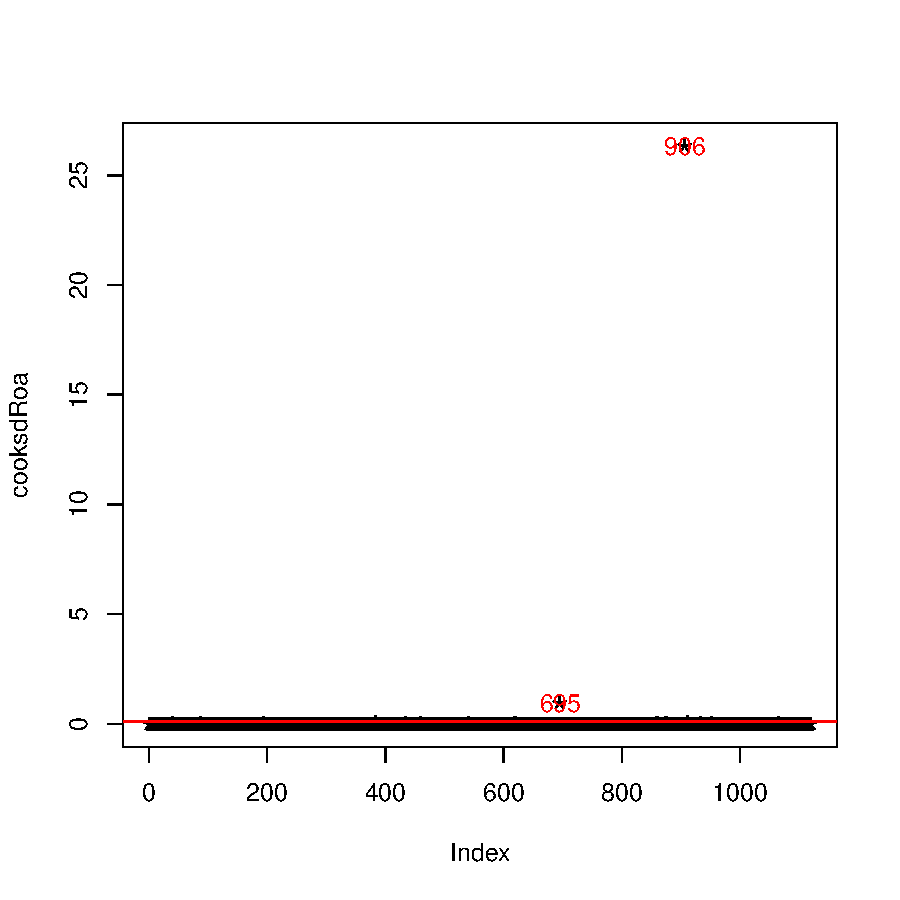
\includegraphics{/figures/unnamed-chunk-28-1} \end{center}

\begin{center}\includegraphics{/figures/unnamed-chunk-28-2} \end{center}

Here the function outlierTest from \emph{car} package gives the most
extreme observation based on the given model. \textbf{Should I remove
those observations from my database?}

\begin{verbatim}
##       rstudent unadjusted p-value Bonferonni p
## 666   9.905081         2.8491e-22   3.3961e-19
## 382  -8.232273         4.8257e-16   5.7522e-13
## 1186 -6.474909         1.3892e-10   1.6559e-07
## 94   -6.465151         1.4786e-10   1.7625e-07
## 481   5.119119         3.5819e-07   4.2696e-04
## 482   5.020838         5.9372e-07   7.0771e-04
## 564  -4.383331         1.2730e-05   1.5174e-02
## 848  -4.379382         1.2959e-05   1.5447e-02
\end{verbatim}

\begin{verbatim}
##       rstudent unadjusted p-value Bonferonni p
## 497  12.101376         1.2047e-31   1.2769e-28
## 499   8.633204         2.1908e-17   2.3222e-14
## 498   6.669377         4.1518e-11   4.4009e-08
## 995   6.227579         6.8476e-10   7.2585e-07
## 1012  6.138307         1.1819e-09   1.2528e-06
## 996   5.989238         2.8948e-09   3.0685e-06
## 819   5.441583         6.5755e-08   6.9700e-05
## 610   4.996946         6.8225e-07   7.2319e-04
## 820   4.387600         1.2620e-05   1.3377e-02
## 818   4.097120         4.5062e-05   4.7765e-02
\end{verbatim}

\FloatBarrier
\newpage
\fancyhead[CO,CE]{Discussion}

\section{Discussion}\label{discussion}

Let's speak\ldots{}

\FloatBarrier
\newpage
\fancyhead[CO,CE]{Conclusion}

\section*{Conclusion}\label{conclusion}
\addcontentsline{toc}{section}{Conclusion}

This is my conclusion\ldots{}

\newpage

\fancyhead[CO,CE]{Appendix}

\section*{Appendix}\label{appendix}
\addcontentsline{toc}{section}{Appendix}

\subsection*{Appendix A : This is an appendix
a}\label{appendix-a-this-is-an-appendix-a}
\addcontentsline{toc}{subsection}{Appendix A : This is an appendix a}

\newpage

\subsection*{Appendix B : This is an appendix
b}\label{appendix-b-this-is-an-appendix-b}
\addcontentsline{toc}{subsection}{Appendix B : This is an appendix b}

\newpage

\fancyhead[CO,CE]{References}

\section*{References}\label{references}
\addcontentsline{toc}{section}{References}

\hypertarget{refs}{}
\hypertarget{ref-Berchicci11PostcardsEdge2007}{}
Berchicci, Luca, and Andrew King. 2007. ``11 Postcards from the Edge.''
\emph{The Academy of Management Annals} 1 (1): 513--47.
doi:\href{https://doi.org/10.1080/078559816}{10.1080/078559816}.

\hypertarget{ref-BenabouIncentivesProsocialBehavior2006}{}
Bénabou, Roland, and Jean Tirole. 2006. ``Incentives and Prosocial
Behavior.'' \emph{The American Economic Review} 96 (5): 1652--78.
doi:\href{https://doi.org/10.1257/000282806779396283}{10.1257/000282806779396283}.

\hypertarget{ref-Chencrosscountrycomparisongreen2018}{}
Chen, Fang, Thomas Ngniatedema, and Suhong Li. 2018. ``A Cross-Country
Comparison of Green Initiatives, Green Performance and Financial
Performance.'' \emph{Management Decision}, February.
doi:\href{https://doi.org/10.1108/MD-08-2017-0761}{10.1108/MD-08-2017-0761}.

\hypertarget{ref-Croissant2008a}{}
Croissant, Yves, and Giovanni Millo. 2008a. ``Panel Data Econometrics in
R: The Plm Package.'' \emph{Journal of Statistical Software} 27 (2):
1--43.

\hypertarget{ref-Croissant2008}{}
---------. 2008b. ``Panel Data Econometrics in R: The Plm Package.''
\emph{Journal of Statistical Software} 27 (2): 1--43.
\url{https://cran.r-project.org/web/packages/plm/vignettes/plm.pdf}.

\hypertarget{ref-Dangsearchrobustmethods2015}{}
Dang, Viet Anh, Minjoo Kim, and Yongcheol Shin. 2015. ``In Search of
Robust Methods for Dynamic Panel Data Models in Empirical Corporate
Finance.'' \emph{Journal of Banking \& Finance} 53 (April): 84--98.
doi:\href{https://doi.org/10.1016/j.jbankfin.2014.12.009}{10.1016/j.jbankfin.2014.12.009}.

\hypertarget{ref-Delmas2015}{}
Delmas, Magali A., Nicholas Nairn-Birch, and Jinghui Lim. 2015.
``Dynamics of Environmental and Financial Performance: The Case of
Greenhouse Gas Emissions.'' \emph{Organization \& Environment} 28 (4):
374--93.
\url{https://pdfs.semanticscholar.org/cbe5/48cbdb9e569de3c79bad22f1f02442374ac8.pdf}.

\hypertarget{ref-DimitriosAsteriou2006}{}
Dimitrios Asteriou. 2006. \emph{Applied Econometrics}.
\url{http://www.macmillanihe.com/page/detail/Applied-Econometrics/?K=9781137415462}.

\hypertarget{ref-Dowell2000}{}
Dowell, Glen, Stuart Hart, and Bernard Yeung. 2000. ``Do Corporate
Global Environmental Standards Create or Destroy Market Value?''
\emph{Management Science} 46 (8): 1059--74.

\hypertarget{ref-Elliott2015}{}
Elliott, Larry. 2015. ``Carney Warns of Risks from Climate Change
'Tragedy of the Horizon'.'' \emph{The Guardian}. September 29.
\url{http://www.theguardian.com/environment/2015/sep/29/carney-warns-of-risks-from-climate-change-tragedy-of-the-horizon}.

\hypertarget{ref-EndrikatMakingsenseconflicting2014}{}
Endrikat, Jan, Edeltraud Guenther, and Holger Hoppe. 2014. ``Making
Sense of Conflicting Empirical Findings: A Meta-Analytic Review of the
Relationship Between Corporate Environmental and Financial
Performance.'' \emph{European Management Journal} 32 (5): 735--51.
doi:\href{https://doi.org/10.1016/j.emj.2013.12.004}{10.1016/j.emj.2013.12.004}.

\hypertarget{ref-HartNaturalResourceBasedViewFirm1995}{}
Hart, Stuart L. 1995. ``A Natural-Resource-Based View of the Firm.''
\emph{Academy of Management Review} 20 (4): 986--1014.
doi:\href{https://doi.org/10.5465/AMR.1995.9512280033}{10.5465/AMR.1995.9512280033}.

\hypertarget{ref-HoffmanClimateChangeStrategy2005}{}
Hoffman, Andrew J. 2005. ``Climate Change Strategy: The Business Logic
Behind Voluntary Greenhouse Gas Reductions.'' \emph{California
Management Review} 47 (3): 21--46.
doi:\href{https://doi.org/10.2307/41166305}{10.2307/41166305}.

\hypertarget{ref-HoughtonClimateChange19951996}{}
Houghton, John T., and Intergovernmental Panel on Climate Change. 1996.
\emph{Climate Change 1995: The Science of Climate Change: Contribution
of Working Group I to the Second Assessment Report of the
Intergovernmental Panel on Climate Change}. Cambridge University Press.

\hypertarget{ref-Hsiao2007}{}
Hsiao, Cheng. 2007. ``Panel Data Analysisadvantages and Challenges.''
\emph{TEST} 16 (1): 1--22.
doi:\href{https://doi.org/10.1007/s11749-007-0046-x}{10.1007/s11749-007-0046-x}.

\hypertarget{ref-HsiaoChapitrePanelData2014}{}
---------. 2014. ``Chapitre 5 : Panel Data Models.'' In \emph{Analysis
of Panel Data}. 54. Cambridge university press.

\hypertarget{ref-JeanJouzel2017}{}
Jean Jouzel. 2017. ``Luxembourg Sustainability Forum 2017 - Jean Jouzel,
Les Enjeux Du Réchauffement Climatique.''

\hypertarget{ref-LiUnderstandingImpactGreen2017}{}
Li, Suhong, Thomas Ngniatedema, and Fang Chen. 2017. ``Understanding the
Impact of Green Initiatives and Green Performance on Financial
Performance in the US.'' \emph{Business Strategy and the Environment},
January, n/a--n/a.
doi:\href{https://doi.org/10.1002/bse.1948}{10.1002/bse.1948}.

\hypertarget{ref-MajumdarRulesDiscretionProductivity2001}{}
Majumdar, Sumit K., and Alfred A. Marcus. 2001. ``Rules Versus
Discretion: The Productivity Consequences of Flexible Regulation.''
\emph{Academy of Management Journal} 44 (1): 170--79.
doi:\href{https://doi.org/10.2307/3069344}{10.2307/3069344}.

\hypertarget{ref-MiroshnychenkoGreenpracticesfinancial2017}{}
Miroshnychenko, Ivan, Roberto Barontini, and Francesco Testa. 2017.
``Green Practices and Financial Performance: A Global Outlook.''
\emph{Journal of Cleaner Production} 147 (Supplement C): 340--51.
doi:\href{https://doi.org/10.1016/j.jclepro.2017.01.058}{10.1016/j.jclepro.2017.01.058}.

\hypertarget{ref-Ng2015}{}
Ng, Anthony C., and Zabihollah Rezaee. 2015. ``Business Sustainability
Performance and Cost of Equity Capital.'' \emph{Journal of Corporate
Finance} 34 (October): 128--49.
doi:\href{https://doi.org/10.1016/j.jcorpfin.2015.08.003}{10.1016/j.jcorpfin.2015.08.003}.

\hypertarget{ref-Park2011}{}
Park, Hun Myoung. 2011. ``Practical Guides to Panel Data Modeling: A
Step by Step Analysis Using Stata.'' \emph{Public Management and Policy
Analysis Program, Graduate School of International Relations,
International University of Japan}.

\hypertarget{ref-PrzychodzenRelationshipsecoinnovationfinancial2015}{}
Przychodzen, Justyna, and Wojciech Przychodzen. 2015. ``Relationships
Between Eco-Innovation and Financial Performance Evidence from Publicly
Traded Companies in Poland and Hungary.'' \emph{Journal of Cleaner
Production} 90 (March): 253--63.
doi:\href{https://doi.org/10.1016/j.jclepro.2014.11.034}{10.1016/j.jclepro.2014.11.034}.

\hypertarget{ref-Scarpellinieconomicfinanceinterface2016}{}
Scarpellini, Sabina, Jesús Valero-Gil, and Pilar Portillo-Tarragona.
2016. ``The `Economicfinance Interface' for Eco-Innovation Projects.''
\emph{International Journal of Project Management} 34 (6): 1012--25.
doi:\href{https://doi.org/10.1016/j.ijproman.2016.04.005}{10.1016/j.ijproman.2016.04.005}.

\hypertarget{ref-Stock2008}{}
Stock, James H., and Mark W. Watson. 2008. ``Heteroskedasticity-Robust
Standard Errors for Fixed Effects Panel Data Regression.''
\emph{Econometrica} 76 (1): 155--74.
doi:\href{https://doi.org/doi:10.1111/j.0012-9682.2008.00821.x}{doi:10.1111/j.0012-9682.2008.00821.x}.

\hypertarget{ref-Torres-Reyna2010}{}
Torres-Reyna, Oscar. 2010. ``Getting Started in Fixed/Random Effects
Models Using R.'' \emph{Data \& Statistical Services. Princeton
University}.

\hypertarget{ref-Wooldridge2008}{}
Wooldridge, J. M. 2008. ``Chapter 15: Instrumental Variables and Two
Stage Least Squares.'' \emph{Introductory Econometrics: A Modern
Approach} 4: 506--45.


\end{document}
